\documentclass[Shakespeare.tex]{subfiles}


\begin{document}

\section{Shakespeare Application}

The purpose of the application is to be able to browse through a Shakespeare play in order to analyze its content, read some specific parts and maybe find related information. To do so the application will consist of the following components. The application was written in the eXist IDE environment and all the code for this application can be found on GitHub link from the introduction. Figure \ref{fig:shakespearemain} shows a screenshot of the Shakespeare application with the available plays listed in order.

\begin{figure} [H]
	\centering
	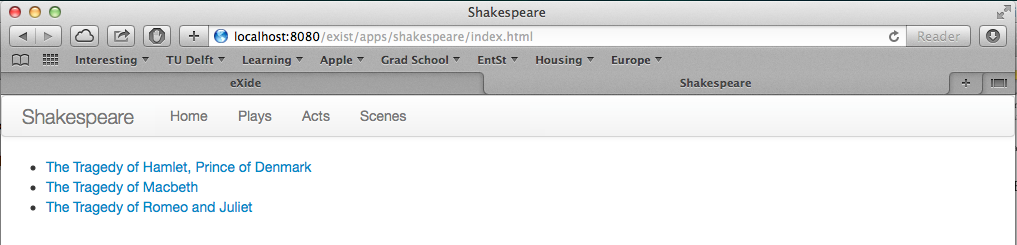
\includegraphics[width=1\textwidth]{./Figures/ShakespeareMain.png}
	\caption{Screenshot of Shakespeare Application}
	\label{fig:shakespearemain}
\end{figure}

\subsection{Architecture}
The architecture for the Shakespeare is detailed below:

\begin{enumerate}
	\item[Pages]
	\begin{enumerate}
		\item Overview of all plays, linking to contents of play
		\begin{enumerate}
			\item Contents of play, includes organization in acts and scenes and characters present in scene
			\item Displaying characters and their parts per act/scene
		\end{enumerate}
	\end{enumerate}
	\item Navigation handler - Decides which page to return based on URL
	\item All scenes and character references appearing link to their respective pages
	\item Navigation Menu
		\begin{enumerate}
			\item Should always include link to full summary of current play
			\item Link to see play overview
		\end{enumerate}
\end{enumerate}

Figure \ref{fig:macbethtoc} below shows the table of contents for Macbeth. The acts, scenes and characters are listed.
\begin{figure} [H]
	\centering
	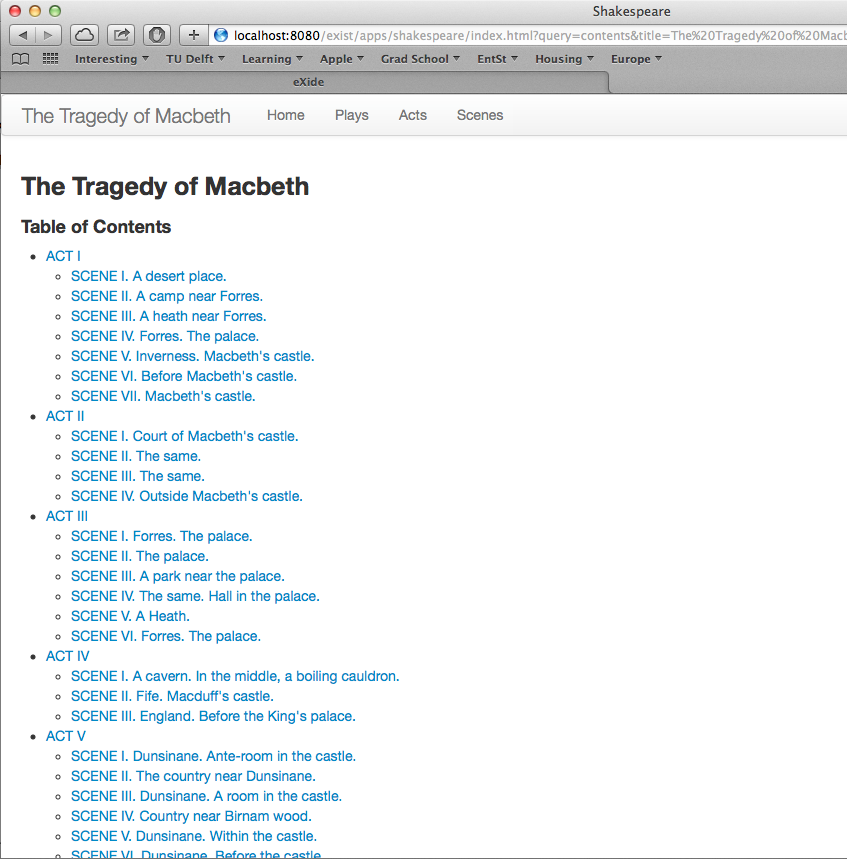
\includegraphics[width=1\textwidth]{./Figures/MacbethTOC.png}
	\caption{Table of Contents for Macbeth}
	\label{fig:macbethtoc}
\end{figure}

\end{document}